\subsection*{Stop, Question, and Frisk data}
After introducing the theoretical tools for assessing fairness, we turn to a case study on the stop-and-frisk practice in NYC. A police officer is allowed to stop a person if they have reasonable suspicion that the person has committed, is committing, or is about to commit a crime.
During the stop the officer is allowed to frisk a person (pat-down the person's outer clothing) or search them more carefully.
The stop can result in a summon, an arrest or no further consequences. After a stop was made, the officer is required to fill out a form, documenting the stop. This data is published yearly by the NYPD.
As mentioned in the introduction the so-called "New York strategy" \cite{gelman2007} is highly controversial. In 2013 how the stop-and-frisk practice was being implemented during 2004 to 2012 in NYC was deemed unconstitutional, violating the fourth and fourteenth amendment {\color{red} Source}

\subsection{Data description}
For our analysis we look at the stops from 2023 as they were the most recent at the time of writing this paper. The raw 2023 dataset consists of 16971 observations and 82 variables. We first discarded all the variables that have more than 20\% missing values, which leaves 34 variables.
From this reduced dataset we filter out the complete cases and end up with 12039 observations. \footnote{Simply discarding the missing values and only training on complete cases is discouraged by \cite{fernando2021}. We opt for this approach regardless, since imputation of the missing values is not straight forward
but treating missing values as an extra category (which some random forest learners in mlr3 can do) will introduce complications when we implement some fairness methods later on.}

% (many fairness methods can not deal with missing data, especially in the protected attribute, which makes sense, since they base their decision on it). 
Race is the protected attribute (PA). For the fairness audit later in the chapter we dichotomize the PA to adjust our situation to the common binary classification, binary PA scenario in the fairness literature. For a more nuanced descriptive analysis we only summarize "Black Hispanic" and "Black" into the group "Black" and  "American Indian/ Native American" and "Middle Eastern/ Southwest Asian" into the "Other" category.  
Black people are by far most often stopped, making up 70\% of the total stops; yet, according to 2020 census data black people make up only 20\% of the city's population \autoref{fig:race_distributions}. At the same time white people form the majority of New York citizens (30\%) but contribute with only 6\% to the stops. 
After 2021 there has been a stark decline in stops and the police is known to focus their attention on high crime areas. Therefore, we further look at each borough. 
The most stops in 2023 occur in Bronx and Brooklyn. Based on report of the NYPD and population statistics from 2020, the Bronx also has the highest estimated crime rate per 100,000 citizens. Manhattan is not far behind in crime rate, but has fewer stops. Note that Bronx and Brooklyn happen to be the boroughs with the highest proportion of black citizens \autoref{fig:nyc_pop_crimerates_stops_comparison}. 
\begin{figure}
  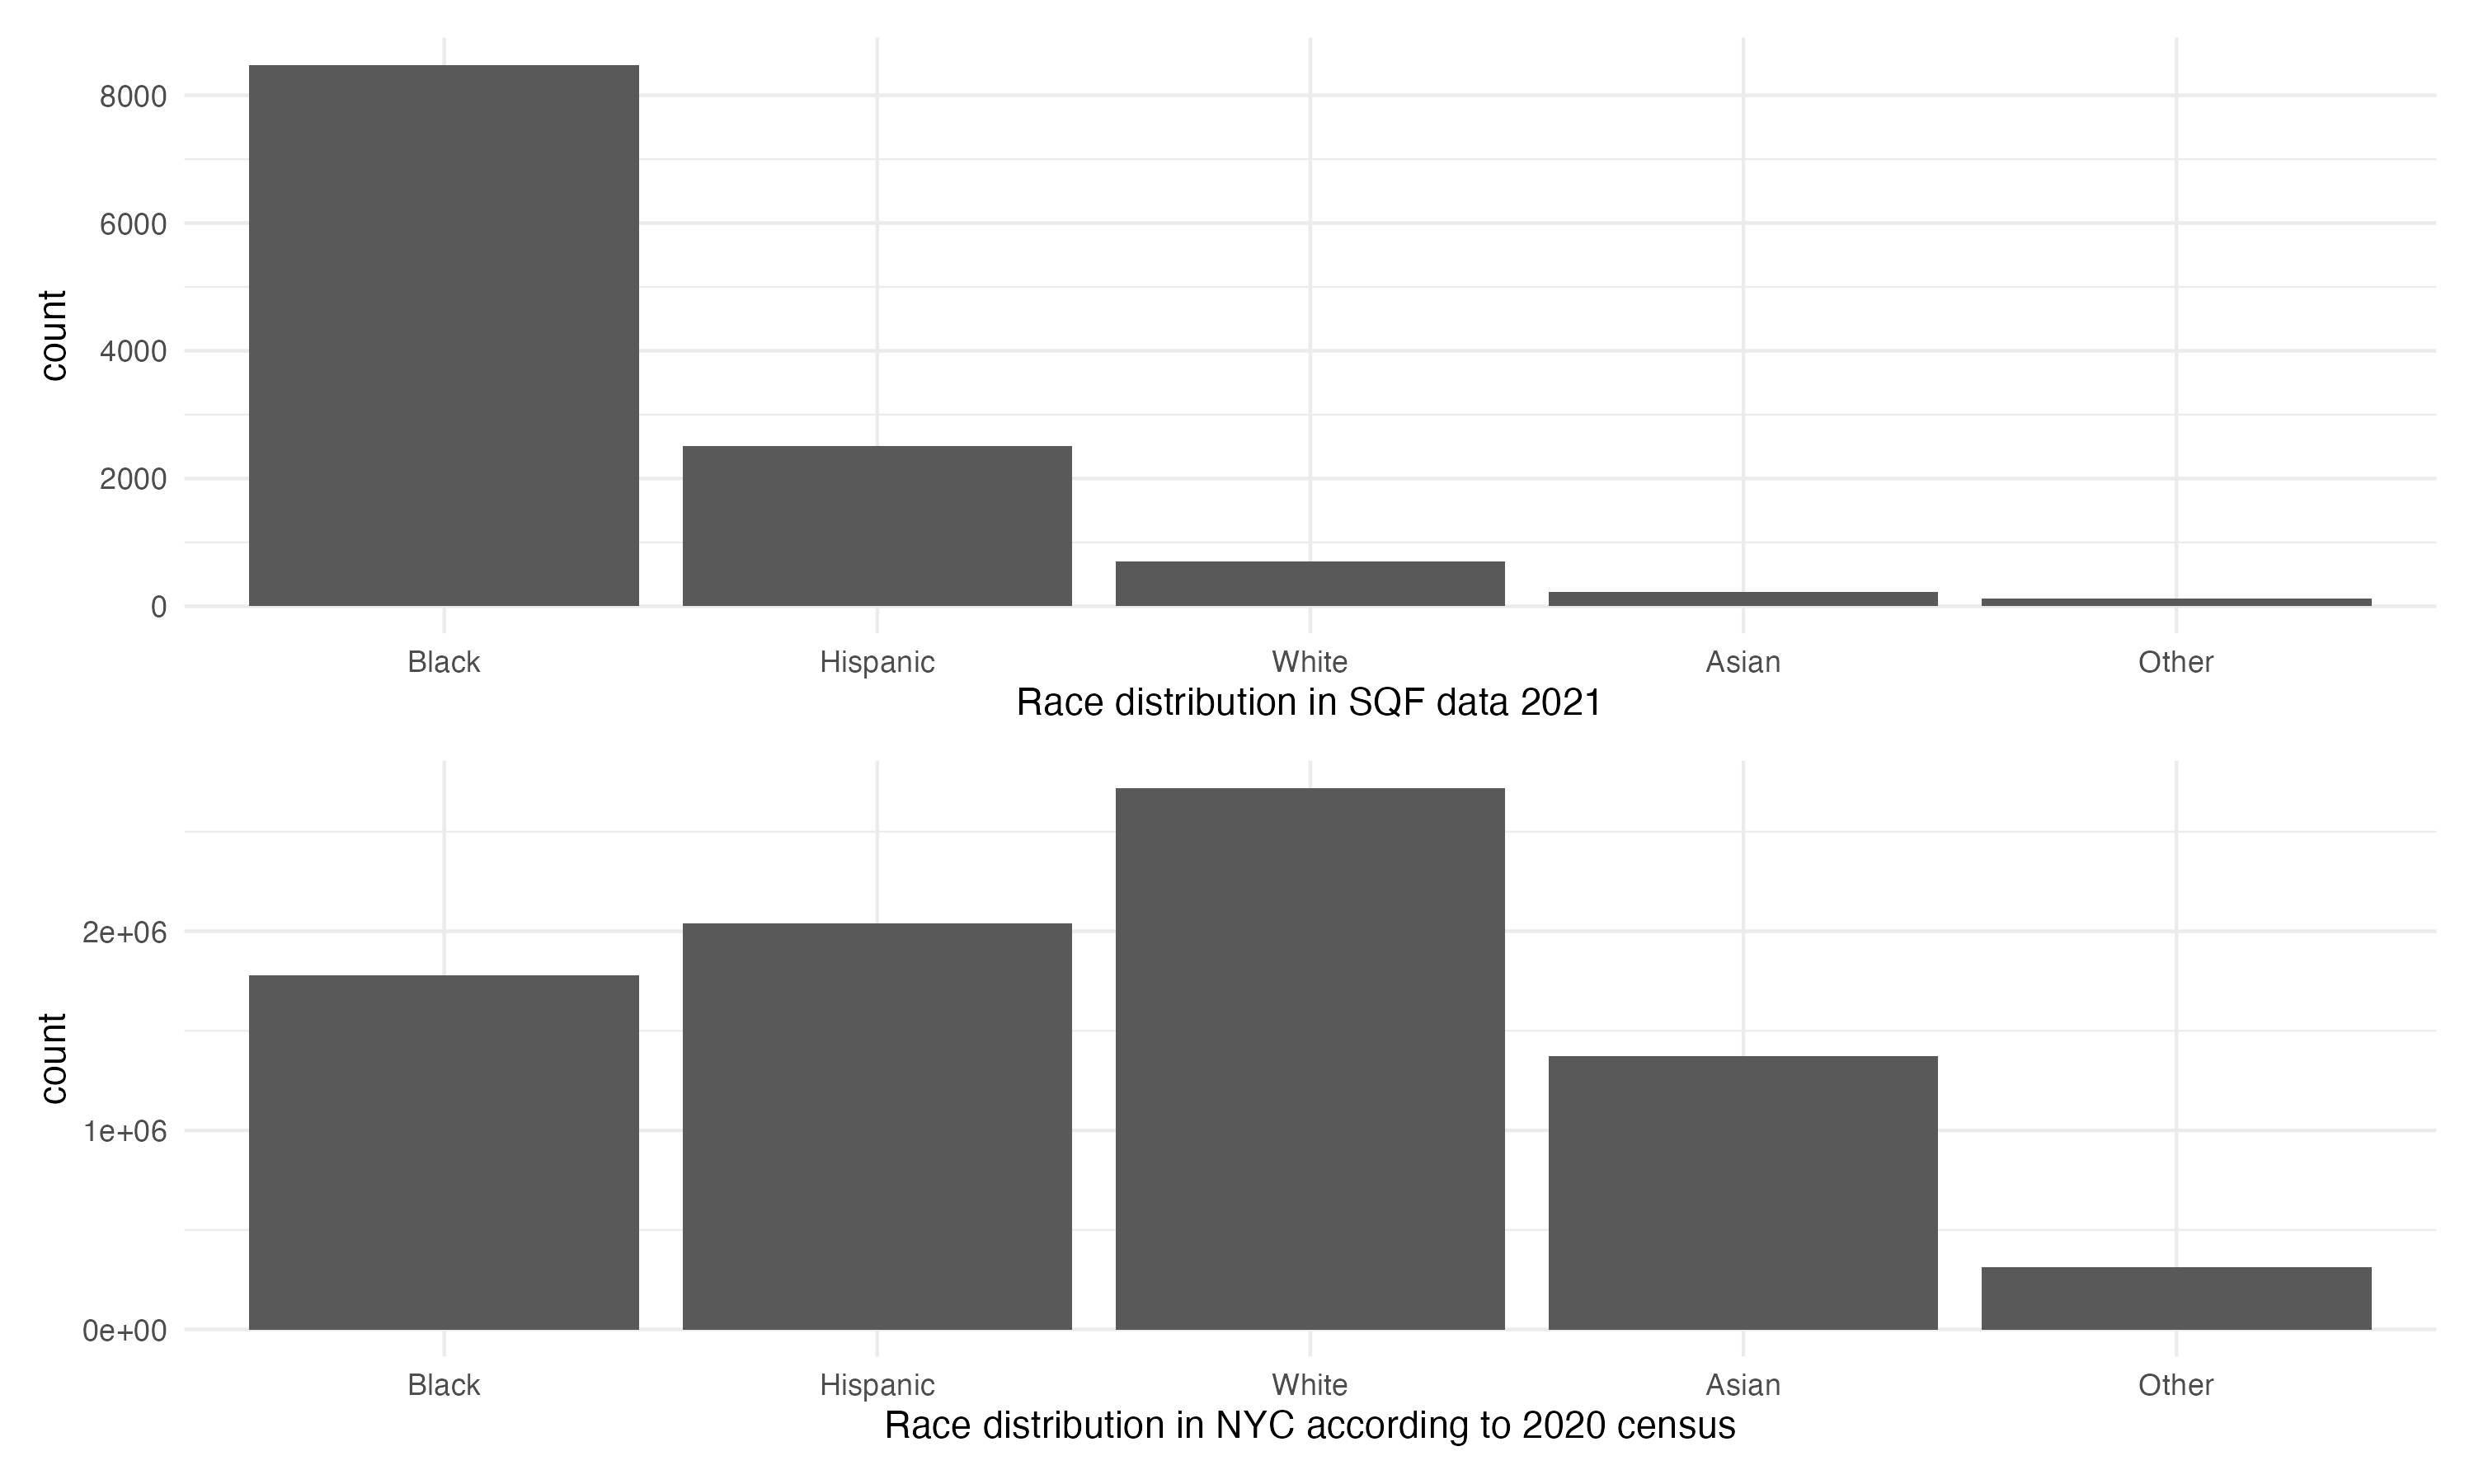
\includegraphics[width=0.5\textwidth]{../figures/sqf_case_study_plot6.png}
  \caption{Comparison of race distribution in the training and target population.}
  \label{fig:race_distributions}
\end{figure}

% \begin{figure}
%     \centering
%     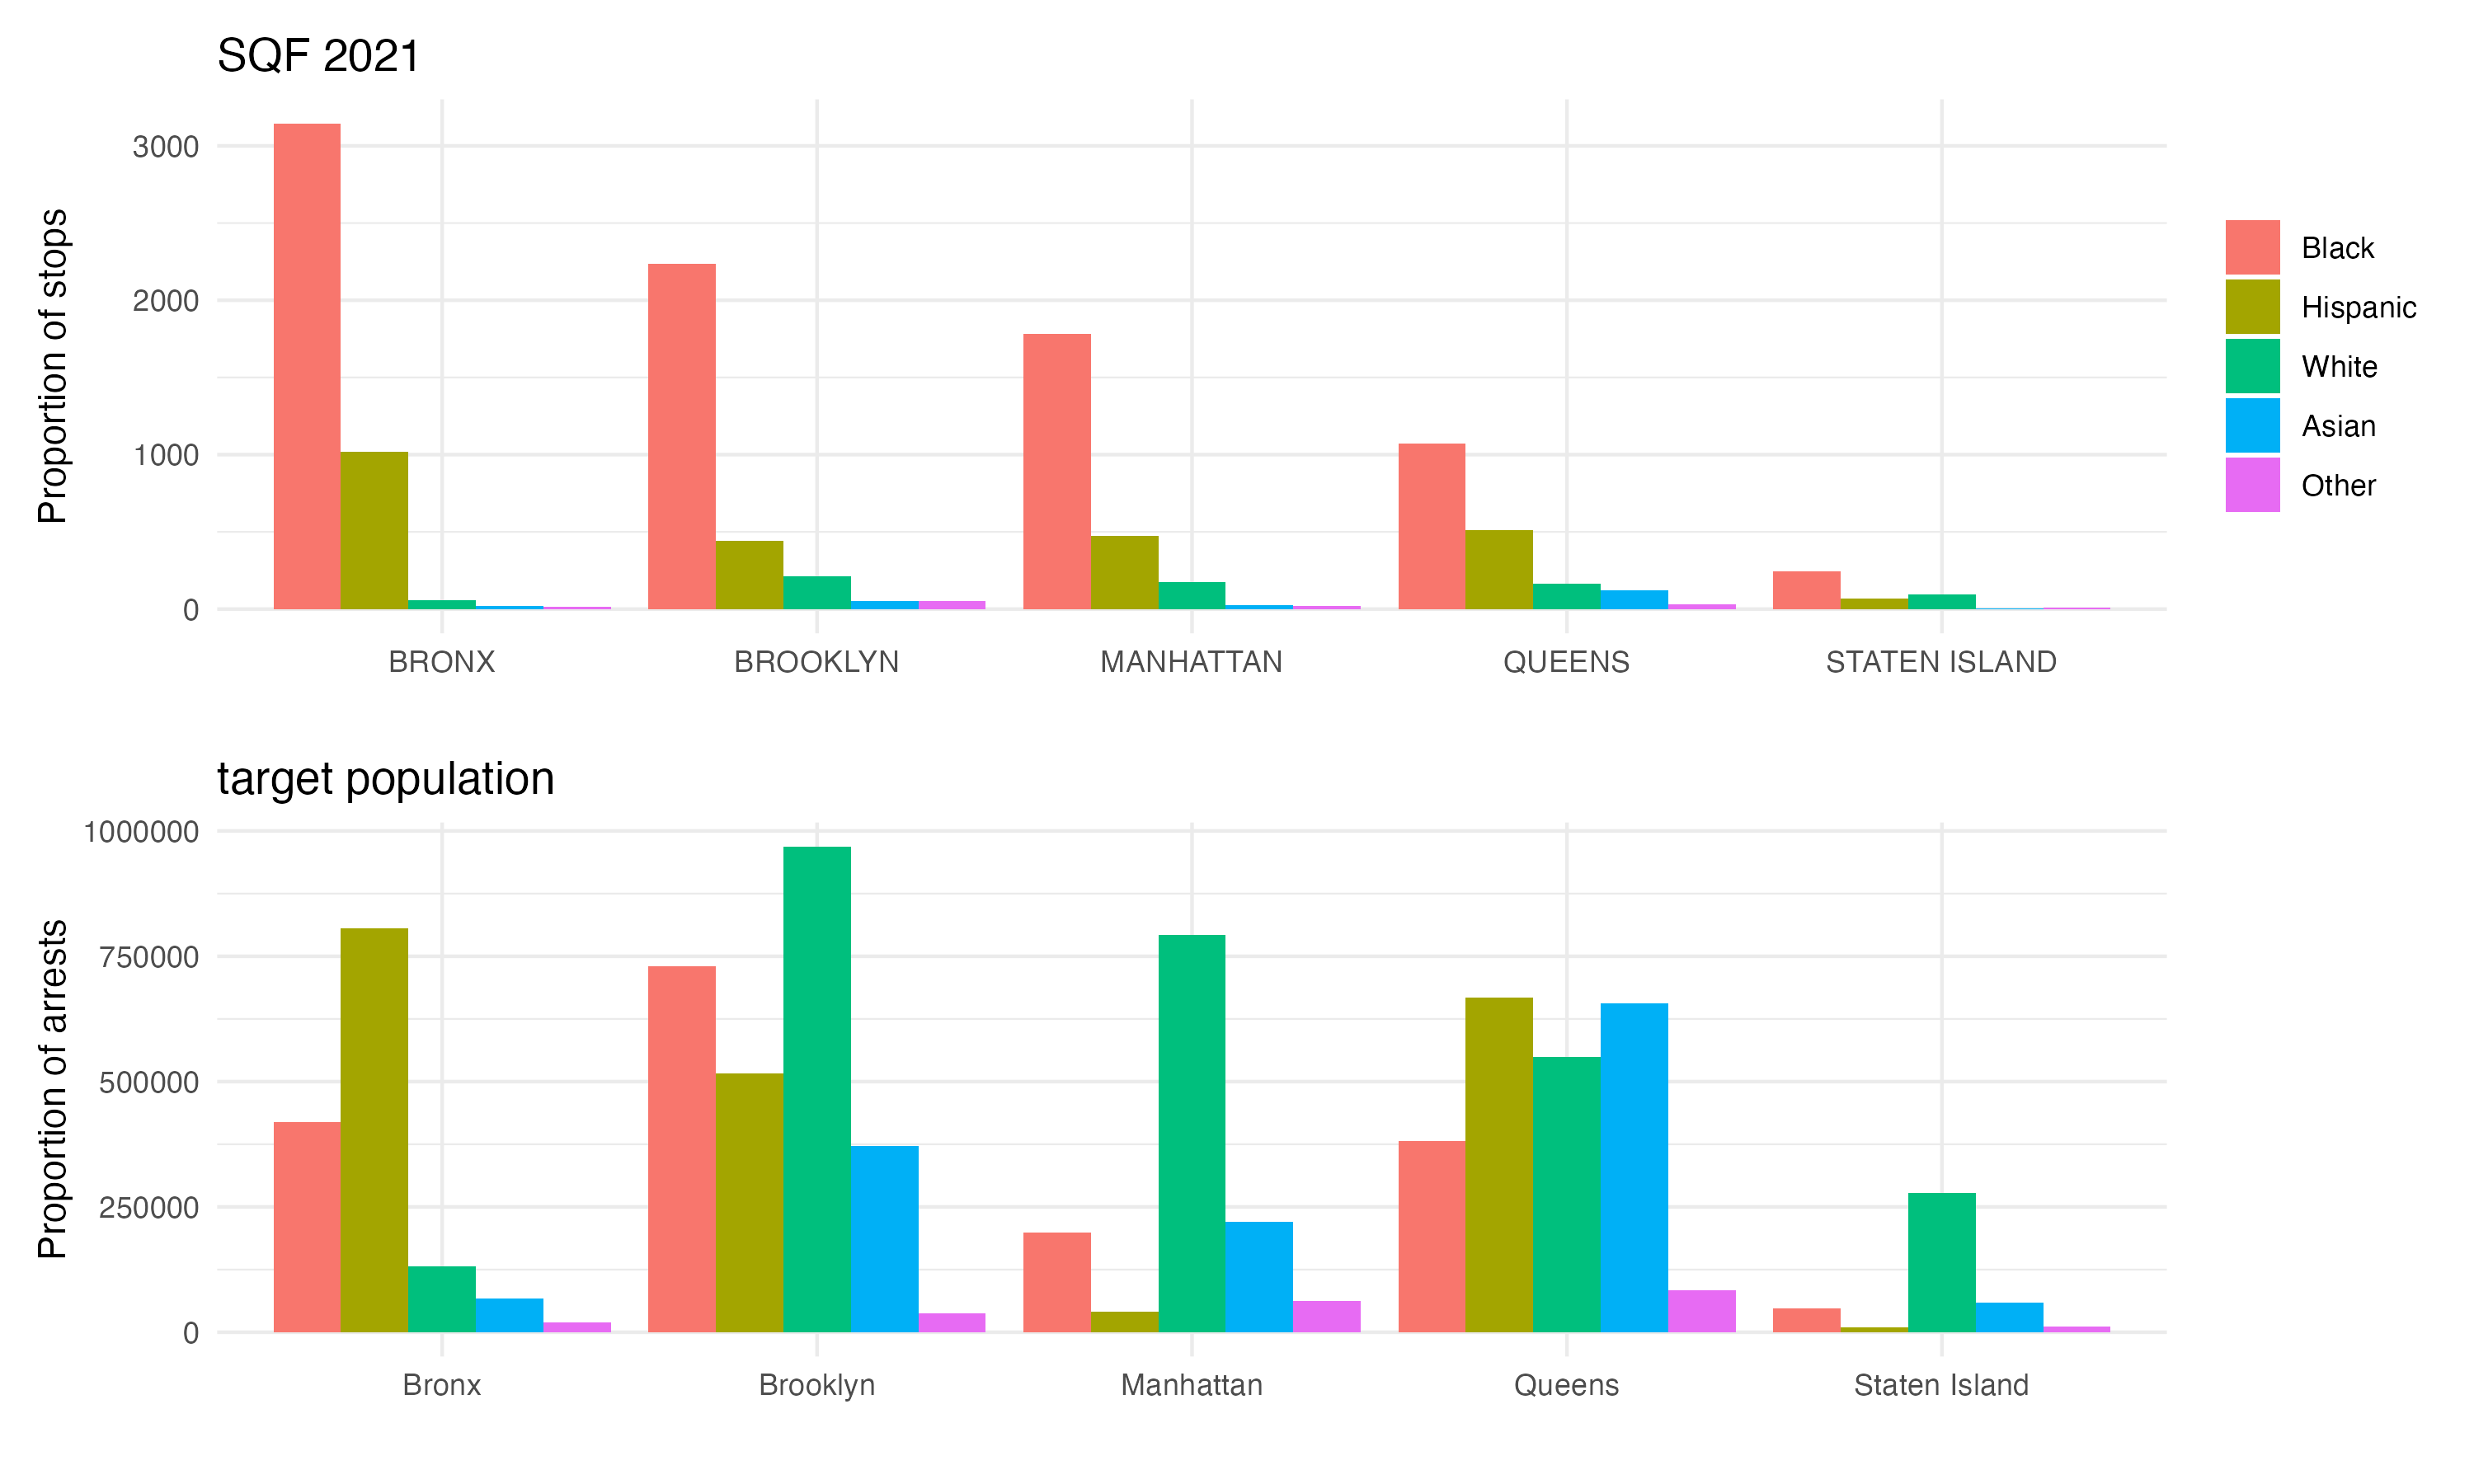
\includegraphics[width=0.7\textwidth]{../figures/sqf_case_study_plot11.png}
%     \caption{Racial distribution in the SQF data of each borough in comparison to the racial distribution of each borough in NYC as a whole.}
%     \label{fig:racial_distribution_borough}
% \end{figure}
\begin{figure}
    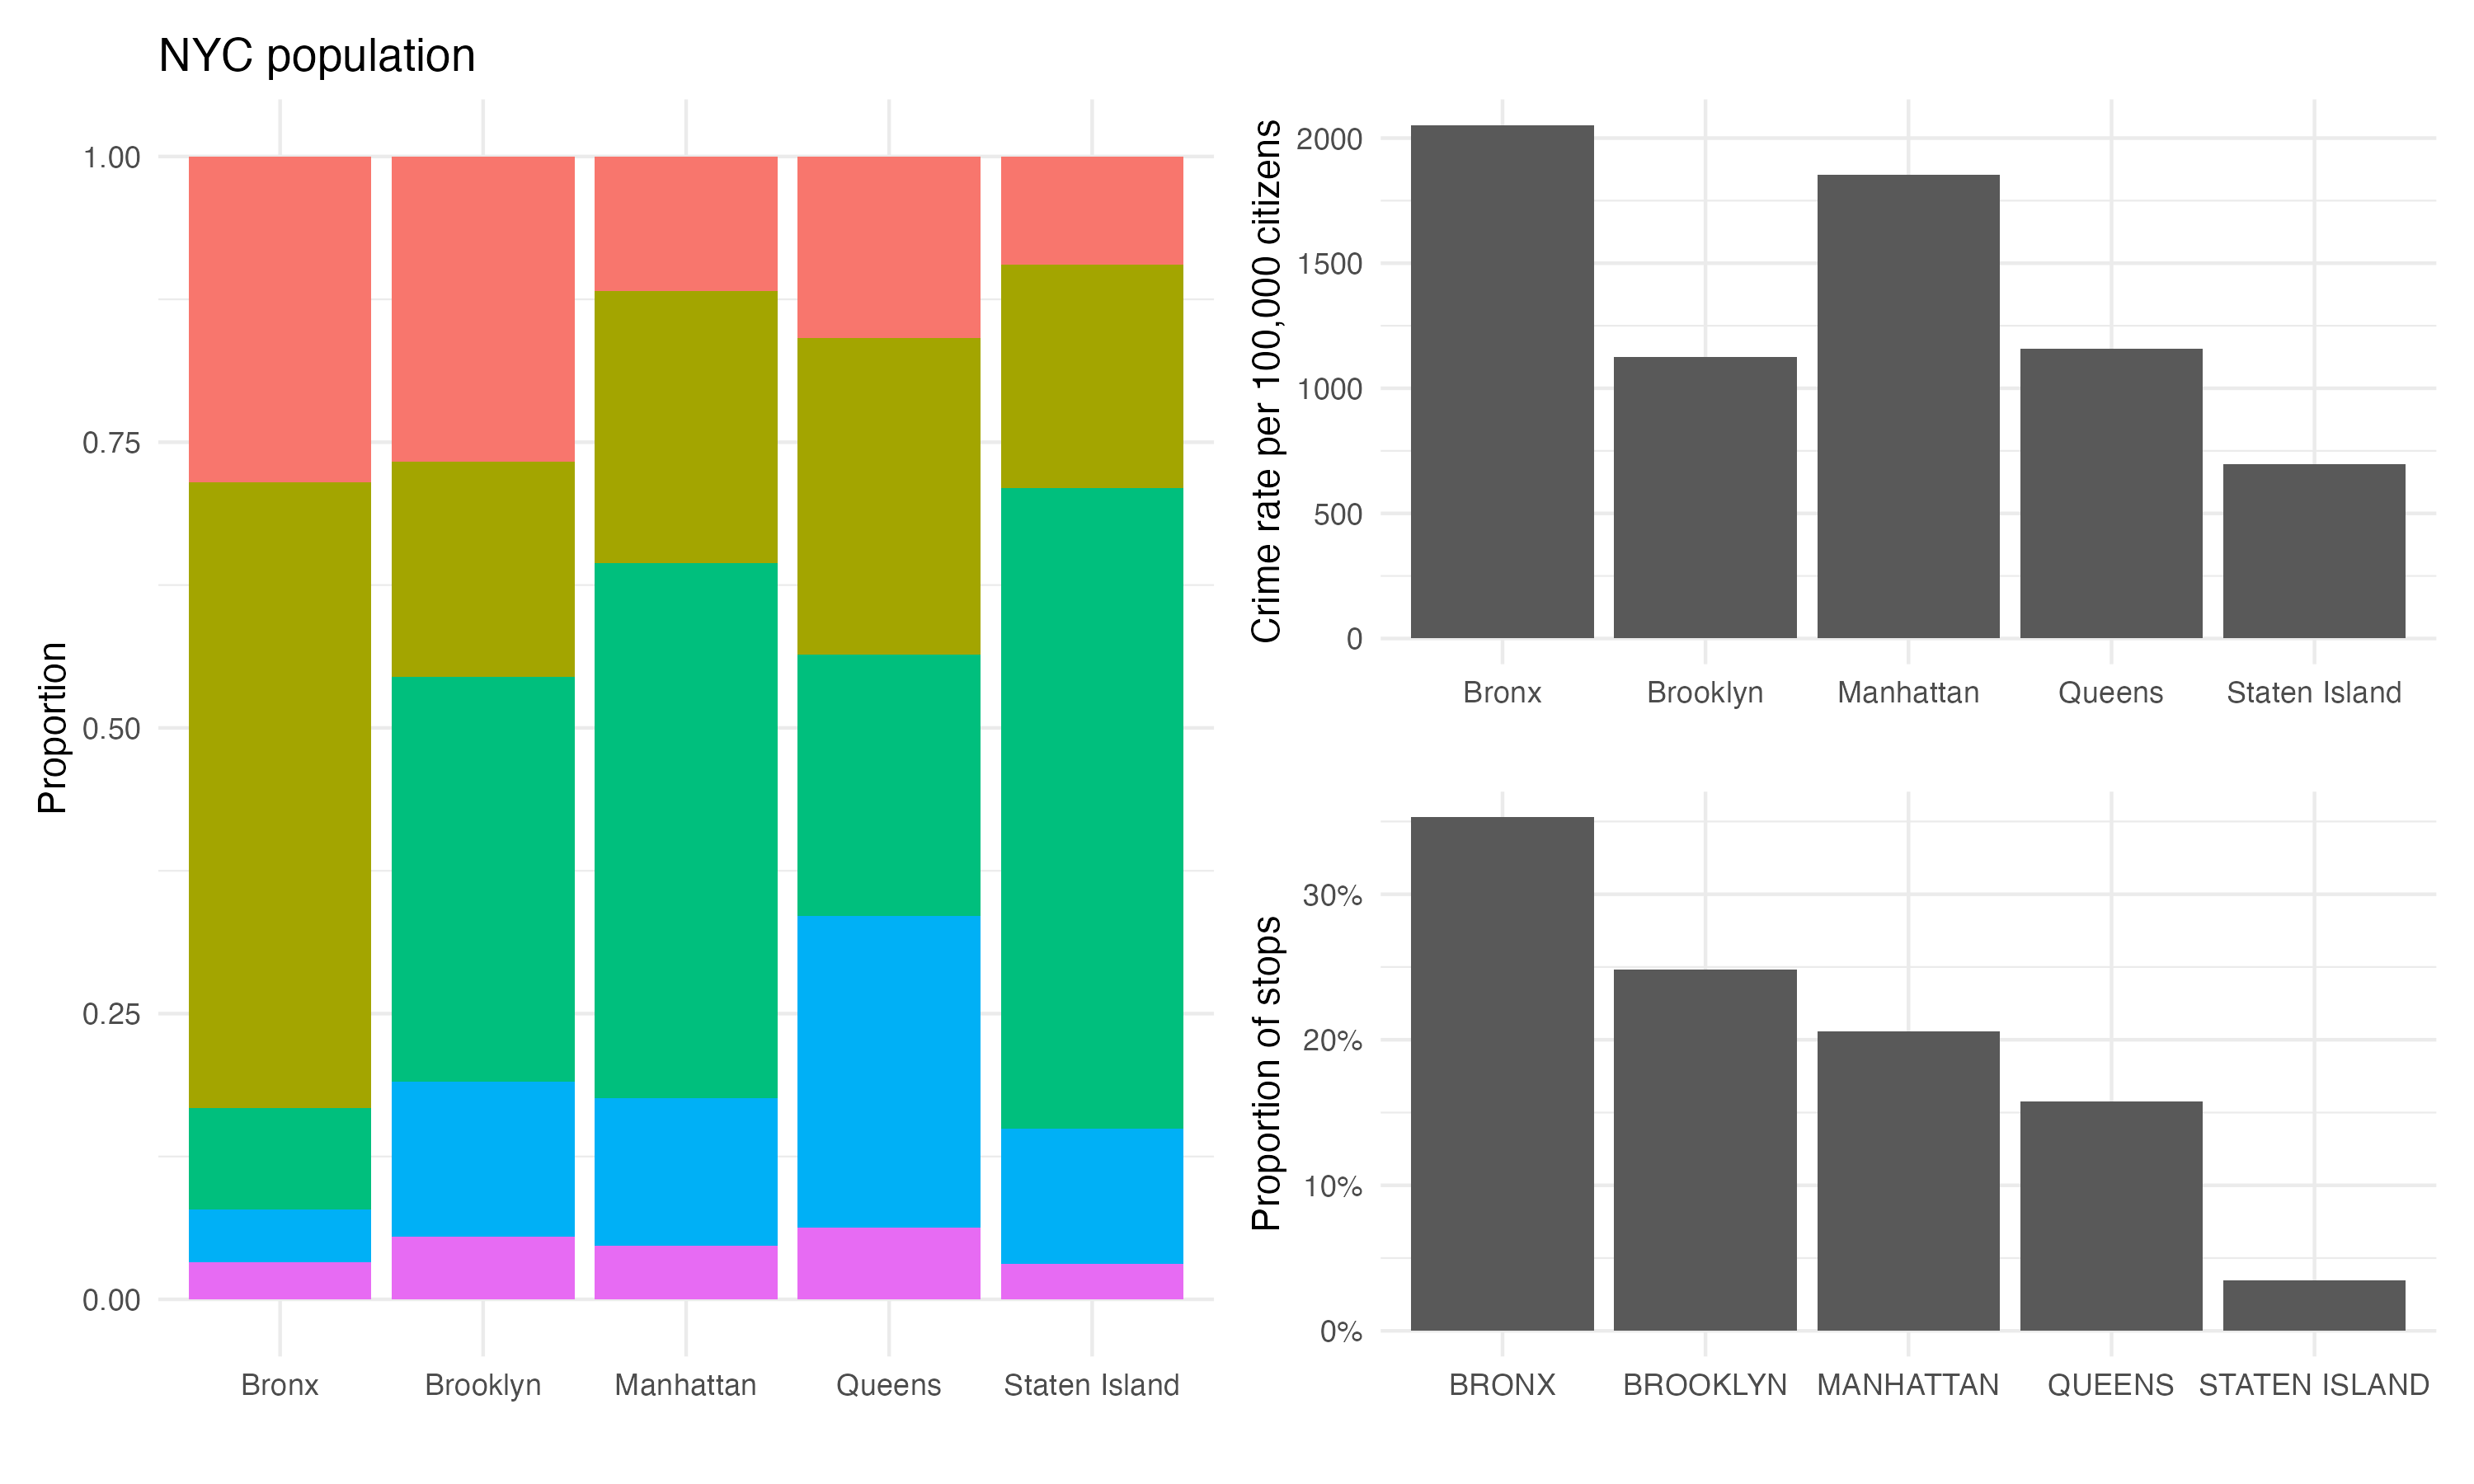
\includegraphics[width=0.5\textwidth]{../figures/sqf_case_study_plot14.png}
    \caption{Estimated borough-wise crime rates (top) versus the proportion of stops in each borough (bottom).}
    \label{fig:nyc_pop_crimerates_stops_comparison}
\end{figure}

After a more general overview of the dataset, we turn to the outcome of the stop. Specifically, we are interested in the arrestment of a suspect. In the cleaned 2023 data about 31\% of stops result in an arrest.
Overall racial disparities in arrestment rates are low. The arrestment rate for white suspects is the highest.
% \autoref{fig:arrestment_rates_clean_data}.
As group fairness metrics are observational and constructed from the joint probability of $Y, \hat{Y}, A$, this already gives us a hint that the classifier trained to predict the arrestment of a suspect might show little racial disparities.

\subsection{Fairness Audit}
To train a random forest classifier on the 2023 data to predict the arrest of a person, we dichotomize the race attribute by grouping "Black" and "Hispanic" as people of colour ("PoC") and "White", "Asian", and "Other" as white ("White").
As features, we select variables that should resemble the information that were available to the officer at the time they made the decision to arrest the person. This includes information about the development of the stop, e.g. whether the person was frisked or a summon issued (we assume that all of these constitute "smaller" hits that happen before an officer chooses the most extreme consequence, an arrest). A full list of the variables in our model can be found in the appendix.
Additionally, we control for factors, such as the time of the stop or whether the officer was wearing a uniform. This selection of features is inspired by previous studies on SQF data (\cite{Badr2022DTFANSP}). With many of the group fairness metrics implemented in \texttt{mlr3fairness}, we can measure the (group) fairness of the regular random forest classifier.\\
First we plot the prediction score densities for each group in \autoref{fig:fairness_density}. We can see that in general white people tend to have higher predicted probabilities than PoC. The mode for the scores for non-white individuals is around 0.05 while it is around 0.125 for white individuals. The score resembles the probability of being predicted positive (arrested).
In \autoref{fig:fairness_metrics} we plot the absolute difference in selected group fairness metrics.
Exact equality of the group metrics cannot be expected in practice, so it is common to allow for a margin of error $\epsilon$. Taking $\epsilon = 0.05$, the classifier is fair according to each of the selected metrics, though the difference in positive predictive rates is close to 0.05.
For a more nuanced picture, we additionally report the group-wise error metrics in \autoref{tab:groupwise_metrics_2023}.
% Interpretation of the direction is, however, not super clear. The positive prediction (to get arrested) is undesirable for the individual, but when a group as a whole has a high proportion of positive predictions, it speaks for the fact that the members were stopped for a good reason. This argumentation follows the principle of assessing a policing strategy based on hit rates. A hit is an arrest and high a high hit rate means that the police is stopping the right people.
% With this ambiguity in mind, we take a closer look at
% We therefore mainly notice the differences in fairness metrics and do not make clear statements about who is discriminated against.
The true positive rate, false positive rate, and the accuracy is basically identical between the two groups. So the Separation metrics are fulfilled. More ore less notable differences can only be seen in the Sufficiency metrics: the negative predictive values/ positive predictive value.


\begin{figure}
    \centering
    \begin{minipage}{0.48\textwidth}
        \centering
        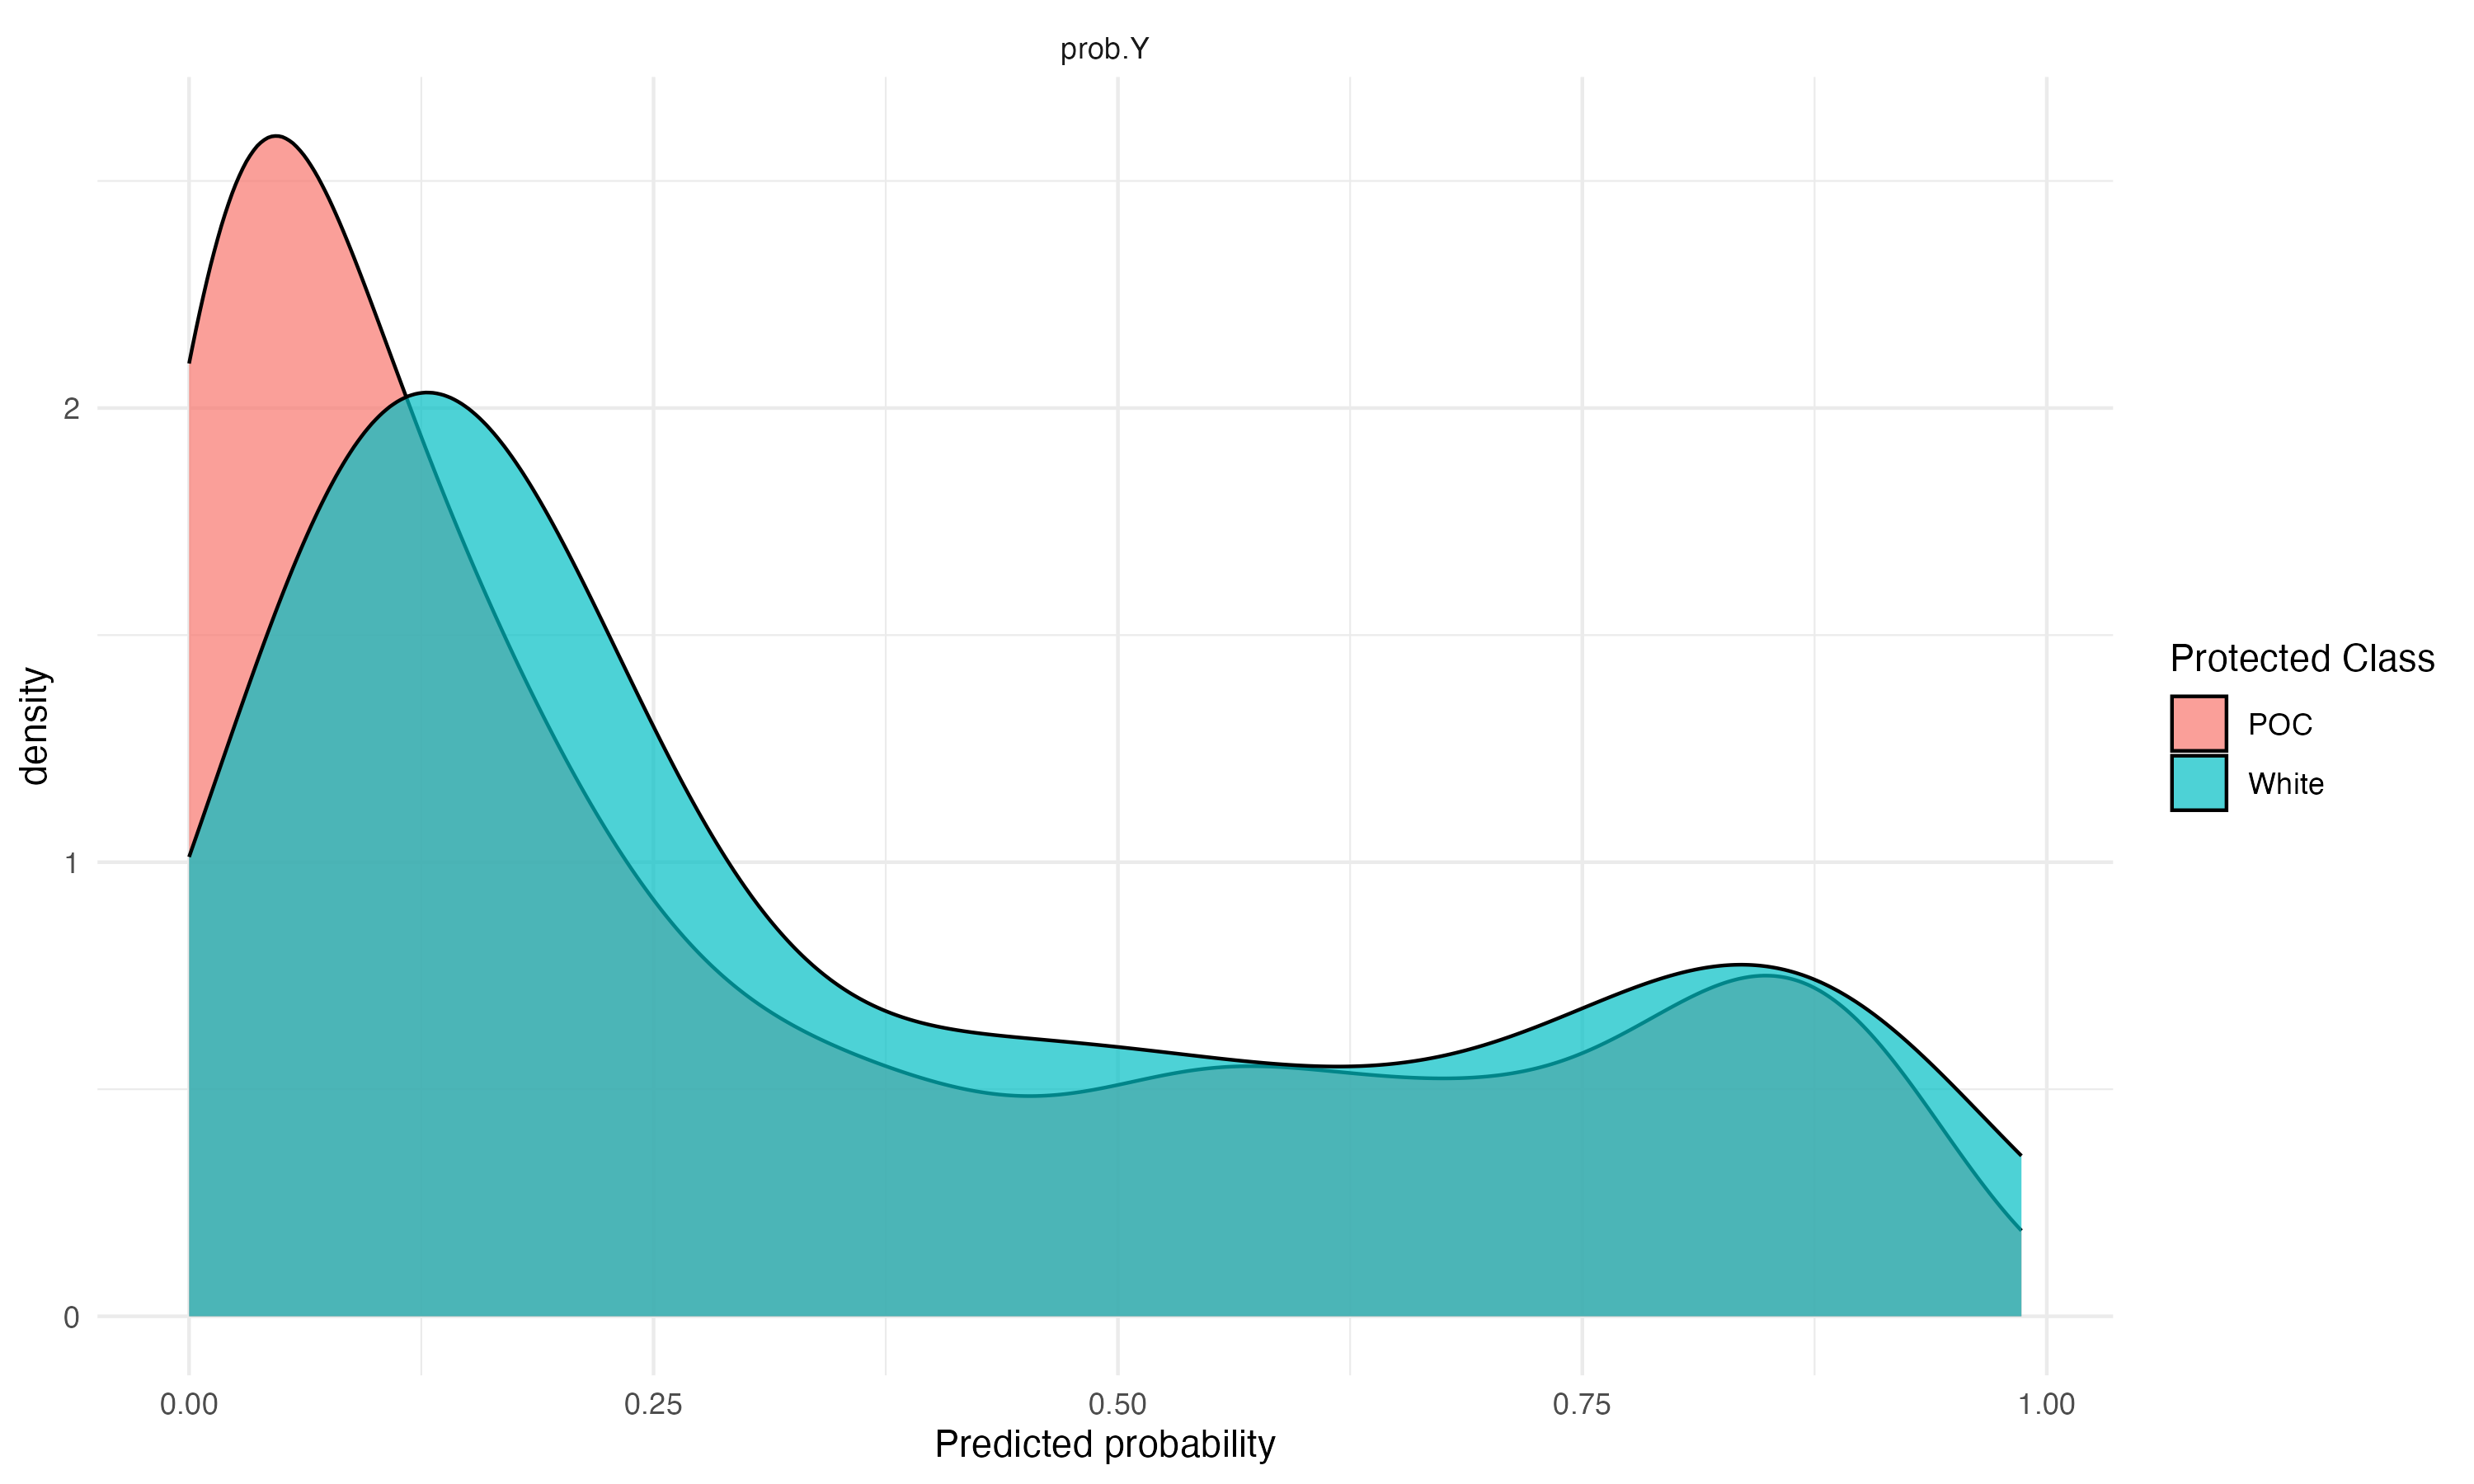
\includegraphics[width=\textwidth]{../figures/sqf_case_study_plot1.png}
        \caption{Density of predicted probabilities for both groups.}
        \label{fig:fairness_density}
    \end{minipage}
    \hfill
    \begin{minipage}{0.48\textwidth}
        \centering
        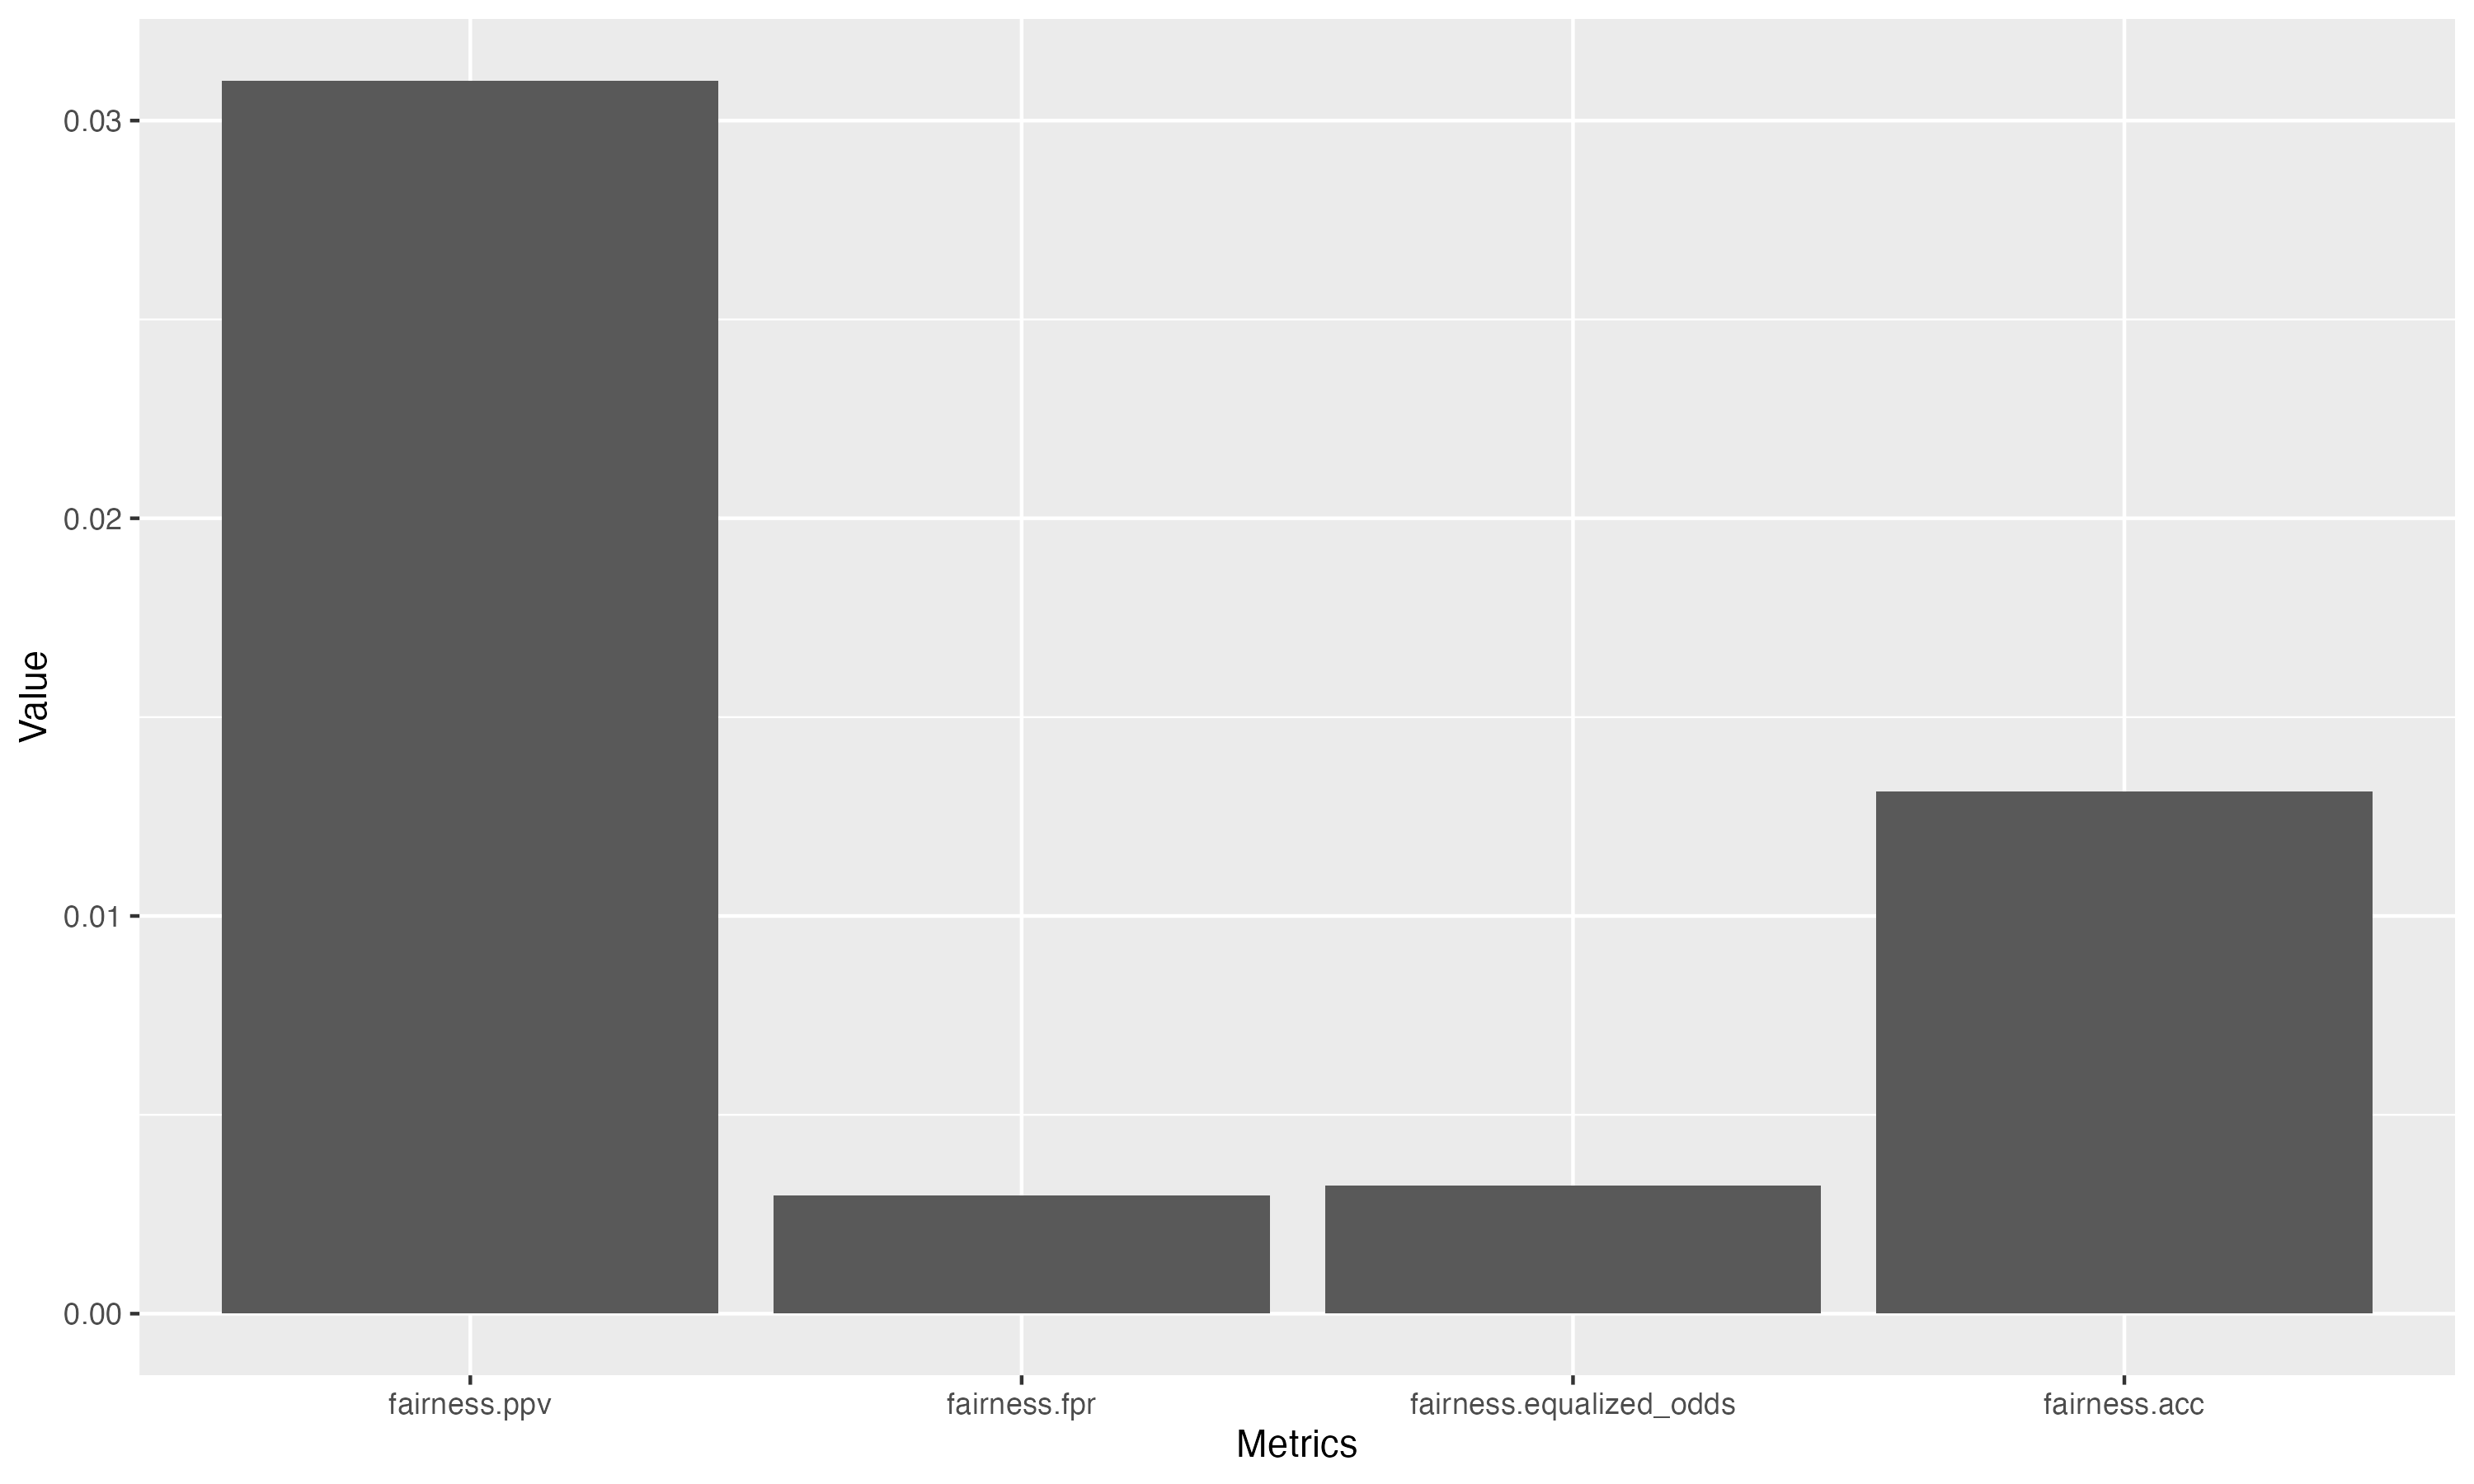
\includegraphics[width=\textwidth]{../figures/sqf_case_study_plot2.png}
        \caption{Another relevant plot.}
        \label{fig:fairness_metrics}
    \end{minipage}
\end{figure}

% results table
\begin{table}[ht]
  \centering
  \begin{tabular}{lrr}
    \hline
  Metric & PoC & White \\ 
    \hline
  tpr & 0.75 & 0.74 \\ 
    npv & 0.89 & 0.85 \\ 
    fpr & 0.07 & 0.06 \\ 
    ppv & 0.84 & 0.89 \\ 
    fdr & 0.16 & 0.11 \\ 
    acc & 0.88 & 0.86 \\ 
     \hline
  \end{tabular}
  \caption{Groupwise Fairness Metrics (2023)} 
  \label{tab:groupwise_metrics_2023}
\end{table}

% \subsubsection*{Fairness Experiment}
% Given that there are indeed disparities for two of the chosen metrics that exceed the $\epsilon$ threshold, we experiment with some fairness methods for the SQF data.
% The \texttt{mlr3fairness} package currently has two pre-processing methods, one post-processing method and some fairness adjusted models implemented. We decide to use a reweighing methods that works with assigning weights to the observations to equalize the distribution of $P(Y|A)$.
% The in-processing method is a fairness-adjusted logistic regression implemented in \texttt{mlr3fairness} inspired by Zafar et al. This method optimizes for statistical parity (Independence). The post-processing method aims for equalized odds, and it works by randomly flipping a subset of predictions with pre-computed probabilities in order to satisfy equalized odds constraints. {\color{red}{reference to mlr3fairness book}} \\
% In \autoref{fig:fairness_experiment} we compare the performance and fairness of each classifier, measured by the difference in true positive rates and the classification accuracy respectively. In the bottom right corner we find fair and accurate classifiers. In terms of fairness reweighing and the equalized odds post-processing method perform best. However, the regular random forest classifier comes close to their fairness performance and performs slightly more accurate. The fairness adjusted logistic regression performs worst in terms of accuracy and fairness.
% As the picture could change depending on the chosen fairness metric (y-axis), we also tried out other metrics, such as equalised odds or predictive parity. In all cases the regular random forest does not perform worse in terms of fairness but better in terms of accuracy than most fairness adjusted classifiers. This supports the in general low racial disparities the fairness audit in the previous section showed.

% % result plot fairness experiment
% \begin{figure}
%     \centering
%     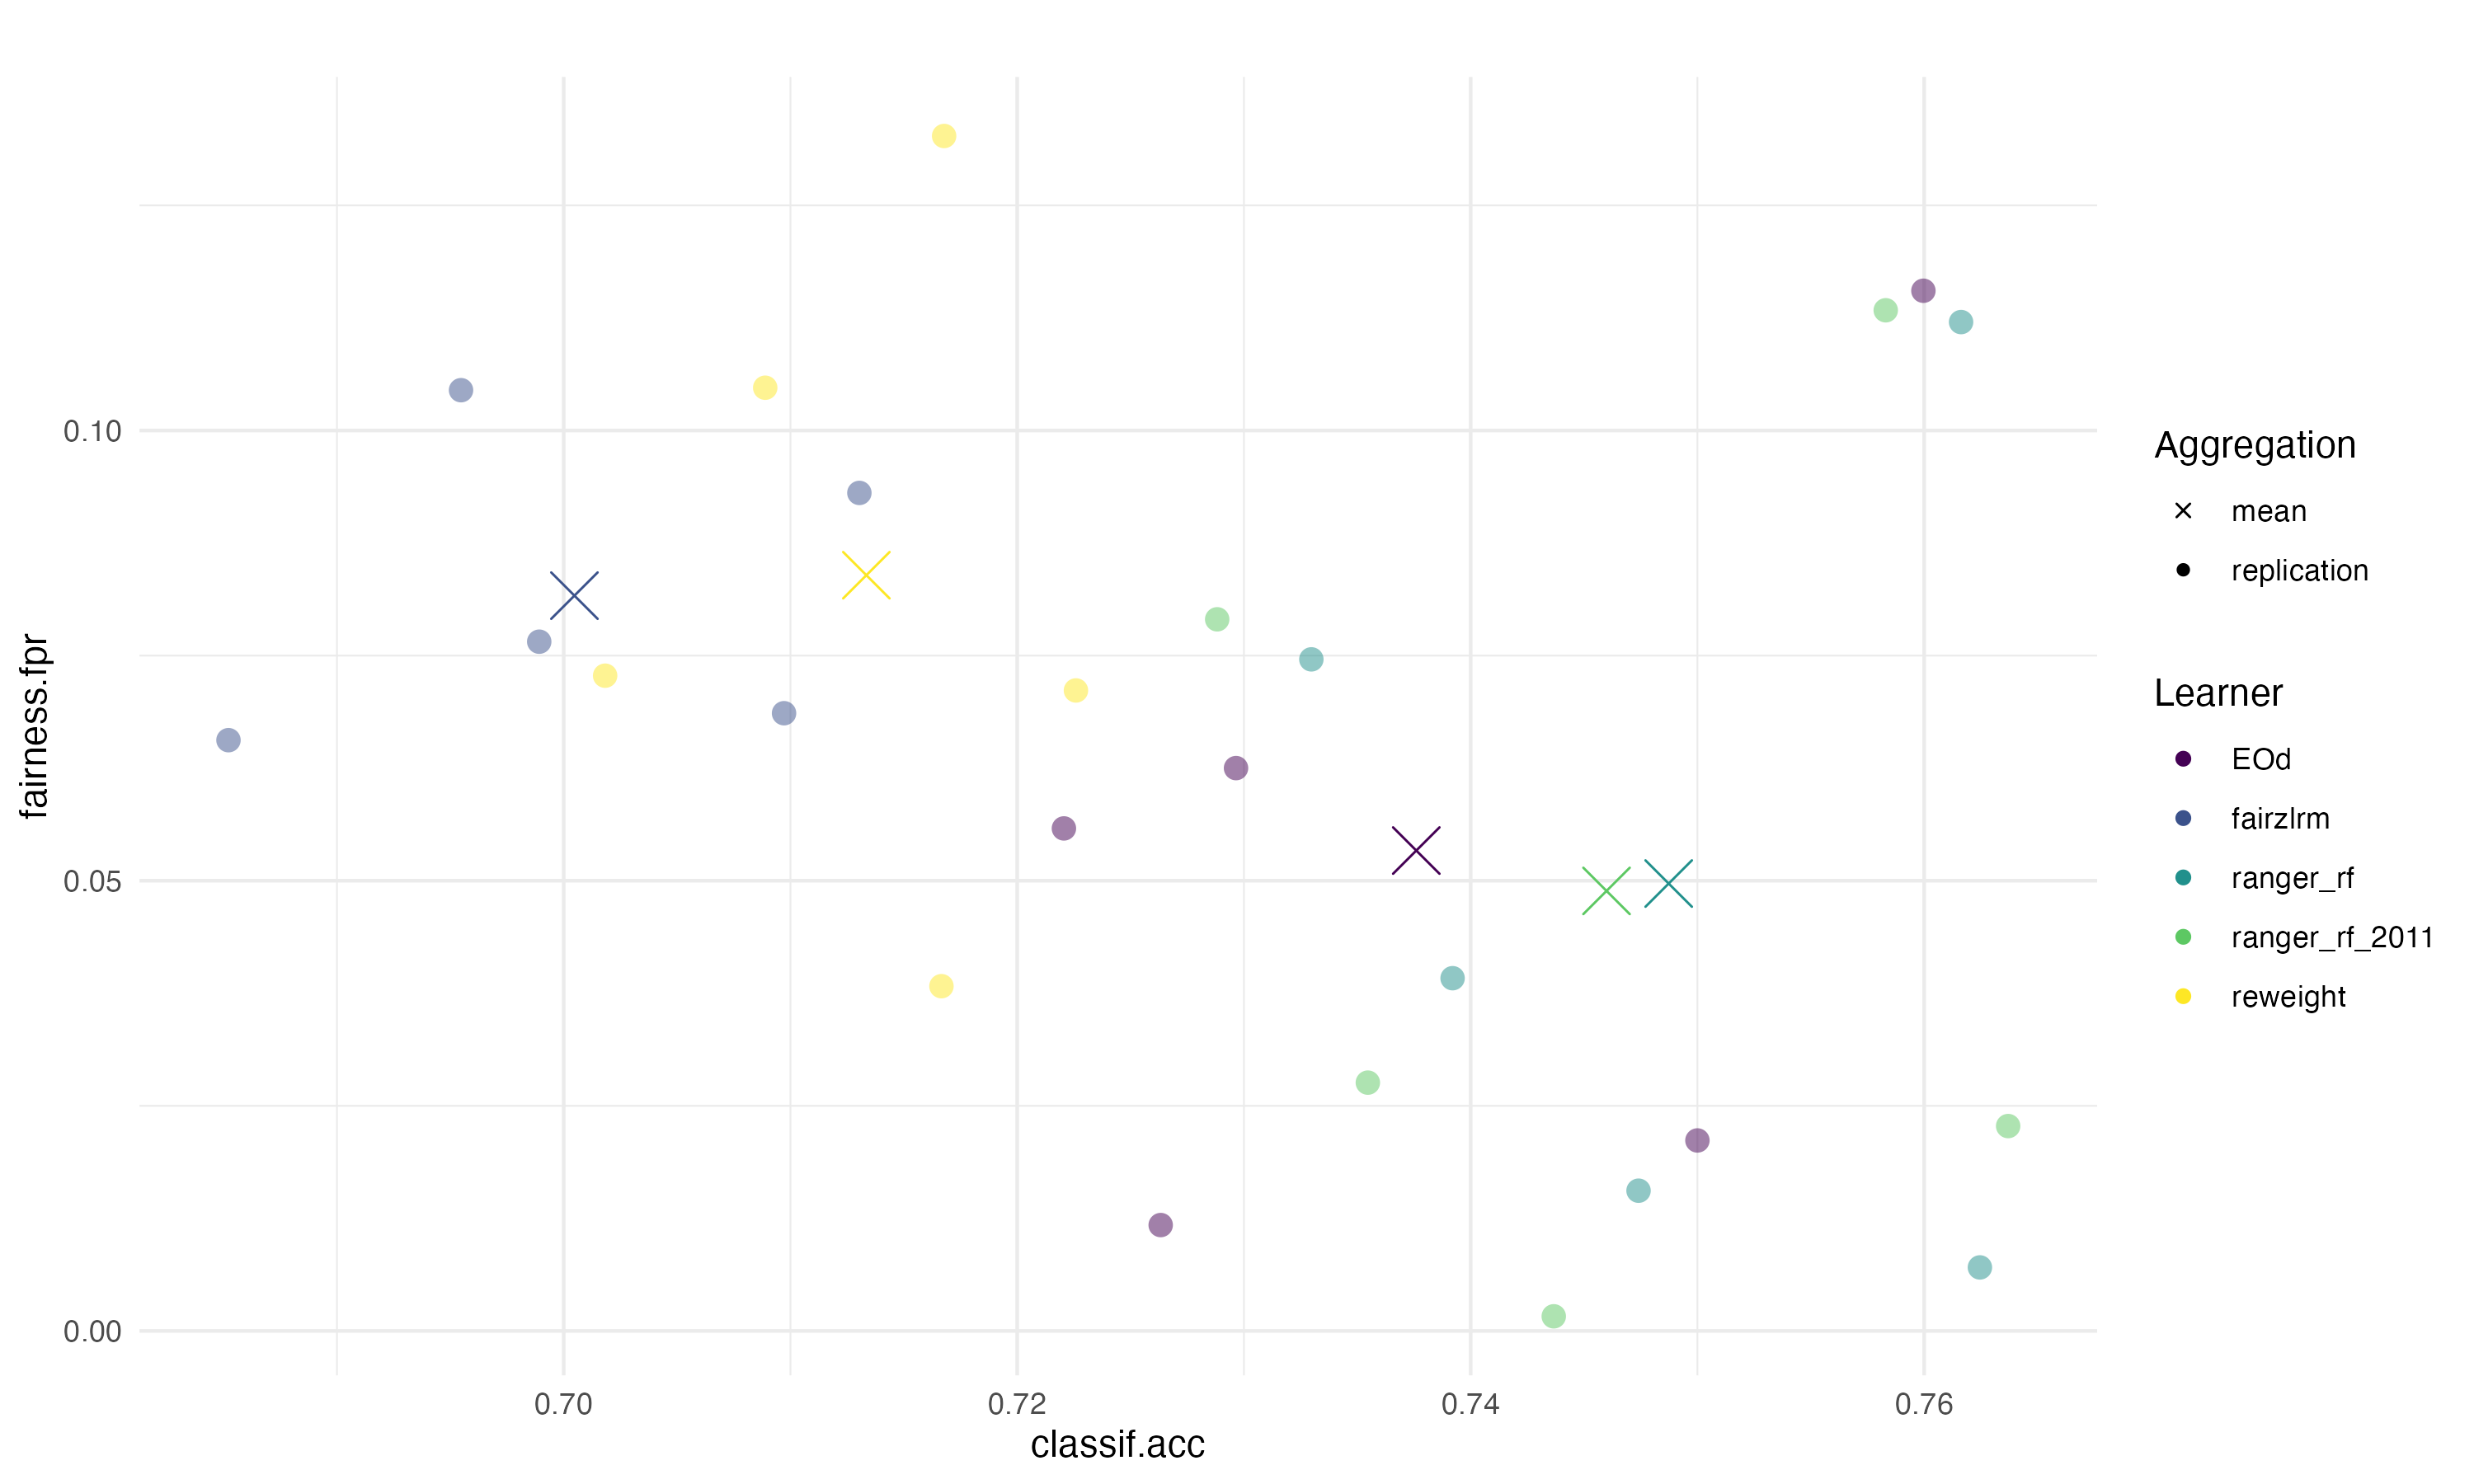
\includegraphics[width=0.7\textwidth]{../figures/sqf_case_study_plot3.png}
%     \caption{Fairness metrics for the fairness adjusted random forest classifier.}
%     \label{fig:fairness_experiment}
% \end{figure}
\subsubsection*{The SQF practice is fair?}
% the other study that supports our results and is contradictory to public belif
All in all, it seems like a classifier trained on SQF data to predict the arrest of a suspect is not discriminatory against PoC. In contrast, it even performs better on many of the common performance metrics for PoC than for white people. This opposes the public belief that the NYPD Stop-and-Frisk practice is biased towards PoC. \cite{Badr2022DTFANSP} have similar findings.
In their study they choose six representative machine learning algorithms (Logistic Regression, Random Forest, XG Boost, GNB, SVC) to predict the arrest of a suspect. Fairness is measured with different metrics (Balanced Accuracy, Statistical Parity, Equal Opportunity, Disparate Impact, Avg. Odds Difference, Theil Index) and separate analysis are conducted with sex and race as PA.
They compare the fairness of the regular learner to the fairness of learner with a pre-processing method (reweighing) and a post-processing method (Reject Option-based Classifier). All in all, they find that the regular models to not perform worse in terms of fairness than the fairness adjusted models. This leads them to conclude "[...] that there is no-to-less racial bias that is present in the NYPD Stop-and-Frisk dataset concerning colored and Hispanic individuals."
What both of our case studies have in common is that the models were trained on recent data. We trained our model on 2023 stops and \cite{Badr2022DTFANSP} used 2019 stops. Since the judgement of how stop-and-frisk was implemented in NYC in 2013, the number of stops has decreased significantly and citizens are in generally less often stopped. After 2014 the stops have been consistently kept at a low level.
\cite{Badr2022DTFANSP} see this as explanation for their results and state "The NYPD has taken crucial steps over the past years and significantly reduced racial and genderbased bias in the stops leading to arrests. This conclusion nullifies the common belief that the NYPD Stop-and-Frisk program is biased toward colored and Hispanic individuals." 



\subsubsection*{Training on stops from an unconstitutional period}
Naturally, the question arises how a classifier trained on data from the unconstitutional period performs.
We choose data from 2011 as it is the year with the most stops. We carry out the same data cleaning steps for the 2011 data as before, starting with 685724 recorded stops and reducing this to 651567 clean observations. Note that these are more than 50 times more stops than in 2023.
The 2011 data has substantially more low-risk stops, only around 6\% of stops result in an arrest. This is a stark contrast to the 2023 data, where 31\% of stops resulted in an arrest.\\
In the data, the differences in arrestment rate between groups are slightly lower for 2011 and the highest arrestment rate remains to be for the white group.
Due to the low prevalence in the population, a classifier trained on 2011 data primarily suffers from the highly skewed distribution of arrests. In terms of fairness, it performs similar to the 2023 classifier.
So somehow the picture is confusing. A classifier trained on SQF data from recent years seems to be fair, and a classifier trained on data from the unconstitutional period is even fairer. In the following we examine alternative approaches to fairness in SQF to find possible explanation.

% Due to the large proportion of low-risk stops in 2011 the predicted probabilities are generally low. In fact, the predicted probabilities for the positive class are generally so low that the classifier rarely predicts the positive class for any person, regardless of group membership.
% A classifier trained on 2011 data primarily suffers from the highly skewed distribution of arrests. A reweighing technique would first need to establish more balance in the target before any fairness analysis becomes relevant.

% Or maybe first a note to the fairness performance of the classifier depended on feature selection.
% Some studies model the ex ante probability of the event, this one models the probability of the event. The difference lies in the features. For learning the ex ante probability the we provide variables to the algorithm that resemble the limited information status of the police officer before the stop, e.g. we specifically do not include the info whether the person was searched or a weapon was found because these are infos the officer get only when they already stopped the person.
% This is what we gave the algorithm. 


% \textbf{Fairness Experiment}
% - fairness metrics (table) for dichotomised race and for full race grouping in appendix.
% - fairness methods (inspired by the article)

% Reweighing: https://mlr3fairness.mlr-org.com/reference/mlr_pipeops_reweighing.html?utm_source=chatgpt.com#format
% Fair logistic regression: https://rdrr.io/cran/mlr3fairness/man/mlr_learners_classif.fairzlrm.html?utm_source=chatgpt.com
% EOd: https://mlr3fairness.mlr-org.com/reference/mlr_pipeops_equalized_odds.html?utm_source=chatgpt.com
% mlr3book: https://mlr3book.mlr-org.com/chapters/chapter14/algorithmic_fairness.html?utm_source=chatgpt.com#bias-and-fairness
% https://mlr3fairness.mlr-org.com/#debiasing-methods



% The data introduced three main challenges: selection bias; missing data; class imbalance.



% borough specific graphics?

% - number of stops conducted but with background information who governed at that time (see Obsidian)
% - transparent explanation of feature selection (similar to Data Transparanecy paper)
% - distribution of race in SQF data vs NYC
% - grouping to black, white, black hispanic, white hispanic, others --> arrestment rates in these groups


